The following components are used for this assignment:

\begin{enumerate}
	\item Raspberry Pi 3 Model B+
	\item Samsung SD Card
	\item Maxim Integrated DS3231 Real Time Clock Breakout Board.
\end{enumerate}

The I2C protocol is used for communications between the RTC and the Raspberry
Pi. As such, the RTC must be connected to the Raspberry Pi via the I2C data and
clock connections, on pins 3 and 5 (GPIO 2 and 3) respectively. The RTC breakout
board operates on a 3.3V supply voltage, and as such the 3.3V (pin 1), and
ground (pin 6) pins must also be connected.

Connecting these pins results in the following layout:

\begin{figure}[H]
	\centering
	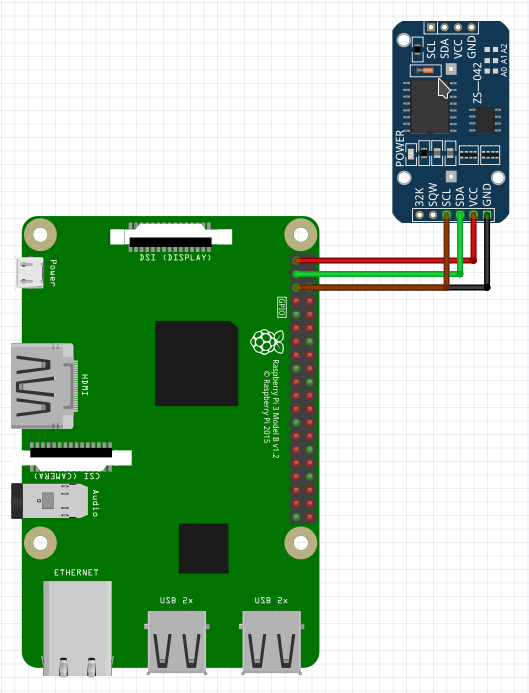
\includegraphics[width=0.45\textwidth, angle=90]{images/circuit}
	\caption{I2C connection from the RTC to the Raspberry Pi}
	\label{fig:images-i2c}
\end{figure}

The physical circuit appears as follows:

\begin{figure}[H]
	\centering
	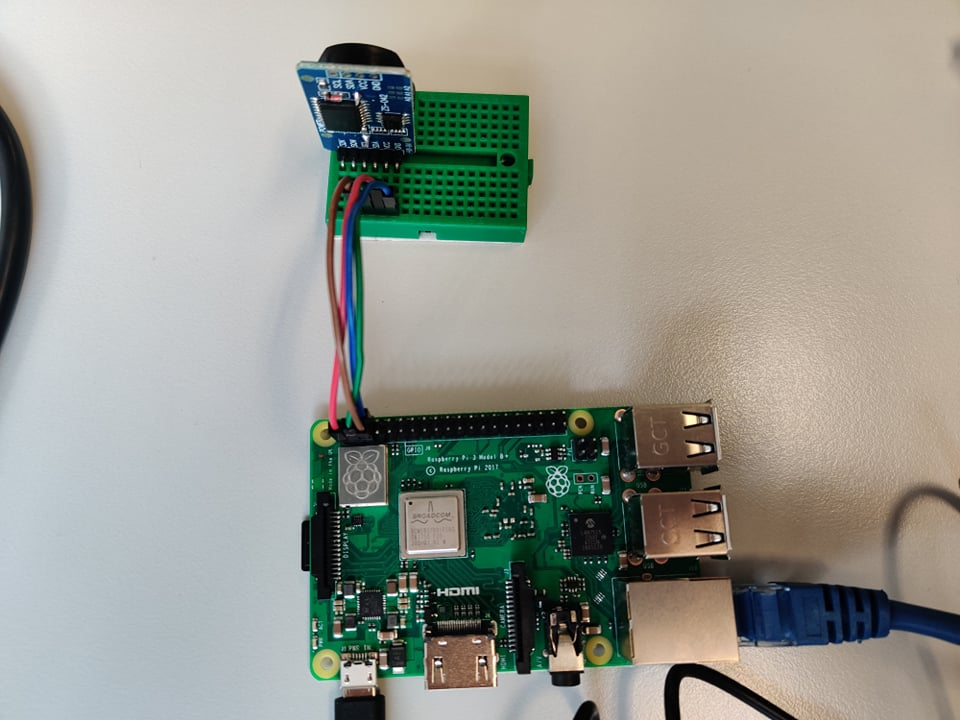
\includegraphics[width=0.8\textwidth]{images/phyCircuit}
	\caption{Physical connection from the RTC to the Raspberry Pi}
	\label{fig:images-phyCircuit}
\end{figure}

The RTC breakout is connected to a breadboard via the connected male header
pins. Four female to male wires connect the Raspberry Pi male GPIO pins to the
breadboard. The wire colours in Figure \ref{fig:images-phyCircuit} are the same
as in Figure \ref{fig:images-i2c}, with the exception of the ground wire, which
in the case of the physical circuit is blue.
